\section{Introduction}
\label{sec:intro}

% QC offers speedups
% - Source of speedup: Oracle, run coherently

Quantum computers offer unique capabilities that can be used to
program substantially faster algorithms compared to those written for
classical computers.
For example, Shor's algorithm \cite{shors} can factorize a
number in polynomial time (compared to the sub-exponential time for the
best known classical algorithm).
It is well known that quantum computers provide quantum supremacy.
Most quantum algorithms are not classically simulatable because of the property;
therefore, they are verified through rigorous \emph{formal methods}.
Many frameworks were proposed to verify quantum algorithms \cite{qhoreusage,qhoare,qbricks,qsepa,qseplocal,VOQC}, 
which essentially established quantum semantic interpretations and libraries in some interactive theorem provers,
such as Isabelle and Coq, to permit quantum program verification, with some tactics for proof automation; but building and verifying quantum algorithms in these frameworks are time-consuming and require human efforts. 
Not to mention that many of these frameworks have no quantum circuit compilers,
so that any verified programs require additional efforts to convert to circuits in other platforms. 
On the other hand, automated verification is an active research fields in classical computation with many frameworks being proposed \cite{HoareLogic,separationlogic,nat-proof-fun,nat-proof,nat-proof-frame,10.1145/3453483.3454087,arxiv.1609.00919,martioliet00rewriting,rosu-stefanescu-2011-nier-icse,rosu-stefanescu-ciobaca-moore-2013-lics,10.1007/978-3-642-17511-4_20,10.1007/978-3-642-03359-9_2}, all of which showed strong results in relieving programmers' pain in verifying classical programs. Is there a way to utilize classical automated verification frameworks in verifying quantum programs?


\begin{figure}[t]
  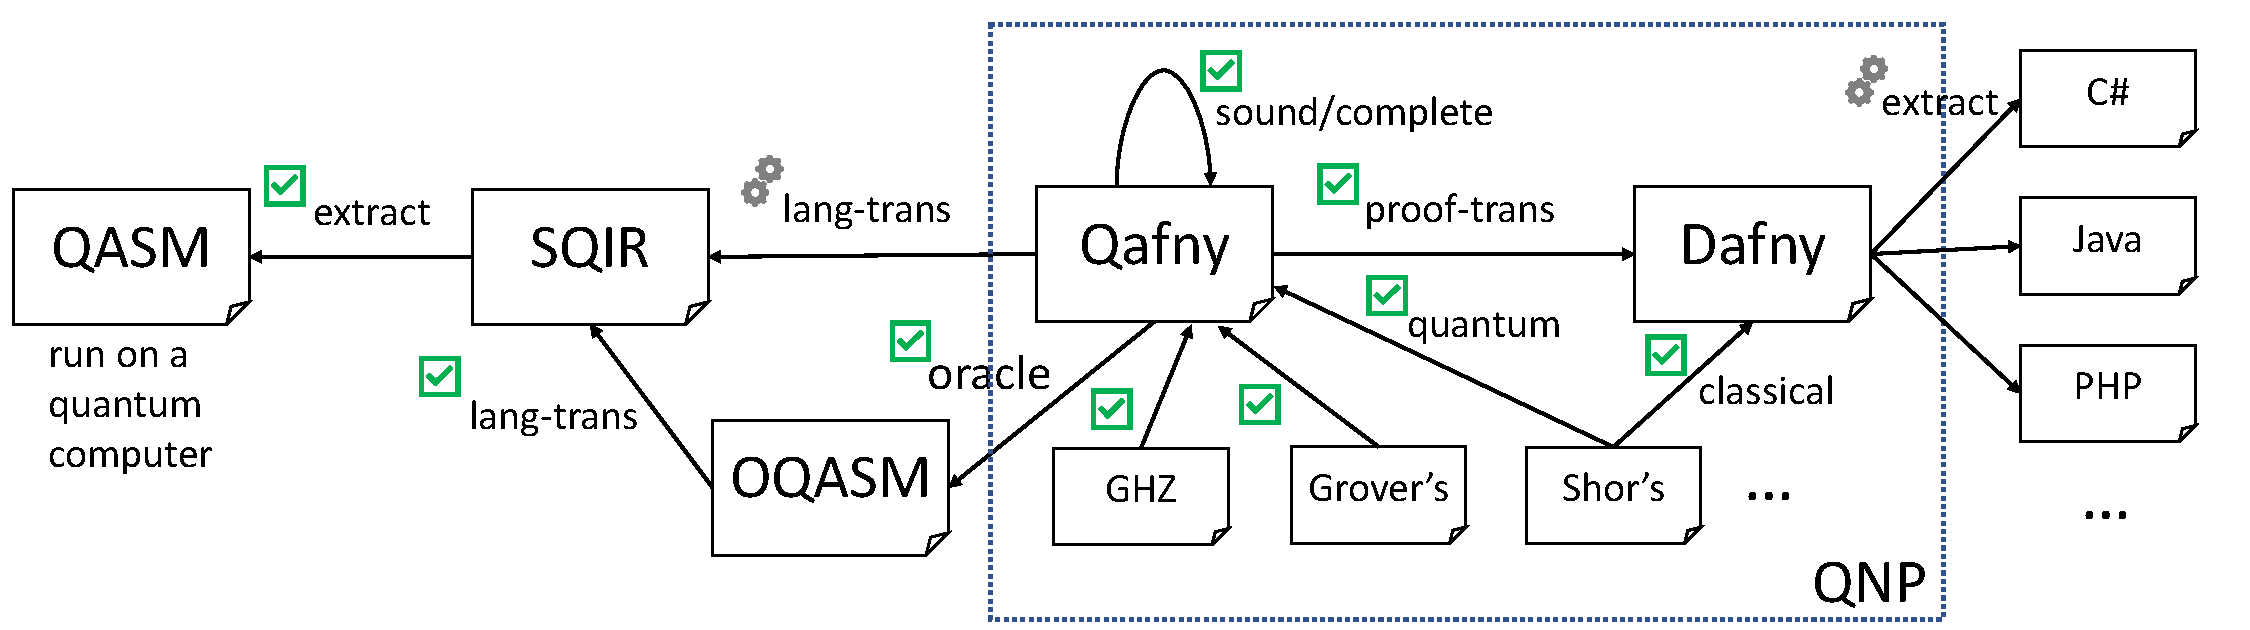
\includegraphics[width=.8\textwidth]{qnp.pdf}
  \caption{QNP Development Stages and the Key Aspects}
\label{fig:arch}
\end{figure}

In this paper, we propose \emph{Quantum Natural Proof} (QNP), a framework that help programmers write and verify quantum programs based on the marriage of quantum program semantics and classical automated verification infrastructure. It has several elements, as shown in \Cref{fig:arch}.

\begin{itemize}
\item Using QNP, an quantum program can be specified in a simple, high-level programming
language we call \qafny, which has standard imperative features and
can express quantum classical hybrid programs with high-level operations,
such as state preparation, oracle, quantum diffusion, quantum conditionals, and for-loops.

\item QNP provides a quantum classical hybird proof system that allows programmers to automatically verify their programs in \qafny.
The quantum portion of the proof system is named the \qafny proof system,
which is specified based on the \qafny quantum language semantics, while the classical part is handled by the Dafny proof system \cite{dafnyref}. 

\item Programmers specify a quantum classical hybrid program specification in QNP. The quantum component verification is relied on the \qafny proof system that translates the quantum part to Dafny and utilizes Dafny's proof infrastructure in finishing the verification,
while the classical component is soley relied on the Dafny proof system.
For examples, GHZ and Grover's searchalgorithms have only quantum components and they are verified by \qafny, while Shor's algorithm is split into quantum and classical components, which are verified by \qafny and Dafny, respectively and collaboratively.

\item The \qafny quantum components can be compiled to quantum circuits and run on a quantum computer via the \qafny to SQIR compiler. 
We compile a \qafny program to SQIR by partially evaluating its classical components, which can be distinguished by the \qafny type system, and only compile its quantum parts to SQIR,  a circuit language embedded in the Coq proof assistant \cite{PQPC,VOQC}.
The quantum compilation has two procedures: 1) quantum oracle operations are compiled to SQIR through an intermediate oracle language \oqasm \cite{oracleoopsla}, and 2) the other quantum components are compiled directly to SQIR. SQIR circuits can be optimized and extracted to OpenQASM 2.0 \cite{Cross2017} to run on a real quantum machine. The \qafny classical components are based on the Dafny infrastructure that can be extracted to several different programming languages, such as C\#, Java and PHP.

\end{itemize}

% OQASM
% - QFT, Eff. simulatable, virtual qubits
% - Proved-correct comp. to SQIR

The key QNP design philosophy leverages the methodology of analogizing quantum operations as classical aggregate operations.
An example that motivates the QNP development is the state preparation in the quantum walk algorithm for Boolean equations \cite{ChildsNAND}, as shown in \Cref{fig:intros-example},
where we first prepare a superposition state $\Msum_{j=0}^{2^n}\ket{j}$ by applying $n$ Hadmard operations (see \Cref{sec:background} for quantum background), then apply an oracle operation $f(\ket{\kappa})=(-i)^{\kappa}\ket{\kappa}$.
If we omit the $\ket{-}$ syntax, the oracle operation is no more than $f(1,\kappa)=((-i)^{\kappa},\kappa)$, where we take the second element $\kappa$ in a pair and push the value $(-i)^{\kappa}$ to the first element.
We can also view the superposition state as an $2^n$ element array; thus, the oracle operation on the state is exactly an array map operation that applies the function $f$ to every array element as shown in \Cref{fig:intro-example-analog}.
What we find out is that most quantum operations can be viewed as some aggregate operations and quantum computers essentially provide an efficient way of applying such aggregate operations.

QNP is designed to reflect the aggregate operation analogy and has two levels of advantages: the programming language and the automated proof system levels. The QNP programming language, \qafny, permits the operation functionality based quantum programs that can be compiled to quantum circuits via the \qafny to \sqir compiler. As a contrast, most quantum programming languages are either built by meta-programs embedded in a host language, such as Python (for Qiskit~\cite{Qiskit}, Cirq~\cite{cirq}, PyQuil~\cite{PyQuil}, and others), Haskell (for Quipper~\cite{Green2013}), or Coq (for \sqir and \voqc \cite{VOQC}), or contain some high level operations with the mix of some circuit gates without a compiler, like \cite{sliqlanguage} and \cite{qsharp}.
In \qafny, we think about program operations as their functionality such as preparing superposition states, applying aggregate oracle operations, quantum conditionals, etc. For example, \Cref{fig:intros-example} is implemented as a state preparation operation, that is compiled to $n$ Hadamard gates, followed by an oracle function $f$. The GHZ \cite{Greenberger1989} implemention in \Cref{fig:background-circuit-example-proof} is a single gate state preparation followed by a for-loop to entangle a list of qubits. 
% by using Hadamard ($\texttt{H}$) and quantum Fourier transform ($\texttt{QFT}$) operations. \Cref{fig:background-circuit-example-proof} Line 2 applies a $\texttt{H}$ operation on $x[0]$, the $0$-th position of the array $x$, but the application can also be applied on the whole array, to prepare superposition of $n$-qubits, as in \Cref{fig:shorqafny}. After the \texttt{H} operator, in the standard implementation of the Greenberger-Horne-Zeilinger (GHZ) circuit \cite{Greenberger1989}, they applies $n-1$ \emph{controlled-not} (\coqe{CNOT}) gates. as shown in \Cref{fig:background-circuit-examplea}. However, in \qafny, we think of \coqe{CNOT} gate's behavior as an application of $n-1$ for-loop steps of quantum conditionals in \Cref{fig:background-circuit-example-proof} line 4-6. In the $j$-th step, the array $x[0..n]$, 



\begin{figure}[t]
  \centering
    \captionsetup[subfigure]{justification=centering}
\begin{minipage}[t]{.5\textwidth}
\subcaption{State Preparation Circuit}
{\quad
  \small
  \Qcircuit @C=0.5em @R=0.5em {
 \lstick{\ket{0}}  & \qw    & \gate{H} & \qw & \multigate{3}{f(\ket{\kappa})=(-i)^{\kappa}\ket{\kappa}}   & \qw &\qw & \qw \\
   &  \vdots &          &     &                                          &    \rstick{\Msum_{j=0}^{2^n}(-i)^{j}\ket{j}} & &\\
   & \vdots  &          &     &                                          &     &       &  \\
  \lstick{\ket{0}} &  \qw   & \gate{H} & \qw &  \ghost{f(\ket{\kappa})=(-i)^x\ket{\kappa}}         &\qw  &\qw    & \qw
    }
}
\label{fig:intros-example}
\end{minipage}
%
\begin{minipage}[t]{.4\textwidth}
\subcaption{State Preparation Analogy}
{
\small
  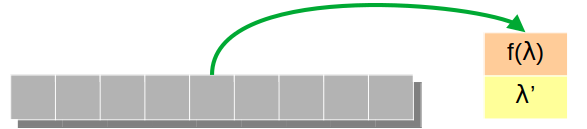
\includegraphics[width=1\textwidth]{oracle}
}
\label{fig:intro-example-analog}
\end{minipage}

\begin{tabular}{c c}
\begin{tabular}{l}
\begin{minipage}[t]{.38\textwidth}
\subcaption{GHZ Circuit}
{\qquad
  \small
  \Qcircuit @C=0.5em @R=0.5em {
    \lstick{\ket{0}} & \gate{H} & \ctrl{1} & \qw &\qw & & \dots & \\
    \lstick{\ket{0}} & \qw & \targ & \ctrl{1} & \qw & &  \dots &  \\
    \lstick{\ket{0}} & \qw & \qw   & \targ & \qw & &  \dots &  \\
    & \vdots &   &  &  & & & \\
    & \vdots &  & \dots & & & \ctrl{1} & \qw  \\
    \lstick{\ket{0}} & \qw & \qw & \qw &\qw &\qw & \targ & \qw
    }
}

\label{fig:background-circuit-examplea}
\end{minipage}
\\
\begin{minipage}[t]{.38\textwidth}
\subcaption{GHZ For-loop Analogy}
{
\small
  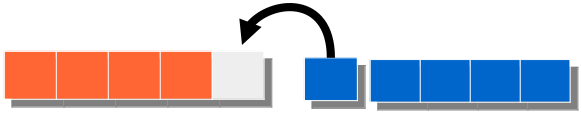
\includegraphics[width=1\textwidth]{ghzforloop}
}
\label{fig:background-circuit-analogy}
\end{minipage}
\end{tabular}
&
\begin{tabular}{l}
\begin{minipage}[t]{.6\textwidth}
\subcaption{\qafny GHZ Program and Proof}
{\small
\[\hspace*{-2em}
\begin{array}{r l}
\textcolor{blue}{1}
&
\textcolor{purple}{
\{x[0..n]\mapsto \ket{\overline{0}}\}
}
\\[0.3em]
\textcolor{blue}{2}
&
\ssassign{x[0]}{}{\ihadh};\\[0.2em]

\textcolor{blue}{3}
&
\textcolor{teal}{
\{x[0..1]\mapsto \frac{1}{\sqrt{2}}(\ket{0}+\ket{1}) * x[1..n]\mapsto \ket{\overline{0}}\}
}
\\[0.3em]

\textcolor{blue}{4}
&
\texttt{for}~{(\texttt{int}~j \in [0,n\,\sminus\,1)~\&\&~x[j])}
\\[0.3em]

\textcolor{blue}{5}
&
\quad
\textcolor{purple}{
\{x[0..\snext{j}]\mapsto \schii{2}{\frac{1}{\sqrt{2}}}{\overline{i}} * x[\snext{j}..n]\mapsto \ket{\overline{0}} * \snext{j} < n\}
}
\\[0.3em]

\textcolor{blue}{6}
&
\quad\;\;
\ssassign{x[\snext{j}]}{}{x[\snext{j}]+1};
\\[0.3em]

\textcolor{blue}{7}
&
\textcolor{teal}{
\{x[0..n]\mapsto \schii{2}{\frac{1}{\sqrt{2}}}{\overline{i}} * x[n..n]\mapsto \ket{\overline{0}}\}
}
\\[0.3em]

\textcolor{blue}{8}
&
\textcolor{purple}{
\{x[0..n]\mapsto \schii{2}{\frac{1}{\sqrt{2}}}{\overline{i}}\}
}
\end{array}
\]
}
\label{fig:background-circuit-example-proof}
\end{minipage}
\end{tabular}
\end{tabular}
\caption{Motivating Examples. $\snext{j}=j\,\splus\,1$. Assume that we have $\kappa\mapsto \schii{2}{}{\overline{i}}$, then $\slen{\kappa}$ is the length of $\kappa$, and $\ket{\overline{i}}$ refers to $m$ number of $i\in[0,1]$ bits, where $m=\slen{\kappa}$. $*$ is the separation conjunction in separation logic. In (d), black parts are \qafny programs, while purple and teal parts are state predicates. }
\label{fig:background-circuit-example}
\end{figure}

The second level is the proof system. While most quantum proof systems, such as QHL \cite{qhoreusage}, QBricks \cite{qbricks},  QSL/BI \cite{qsepa}, and QSL \cite{quantumseparation}, built proof systems based on quantum computation theories, QNP tries to connect the \qafny proof system to traditional separation logic systems; thus, we can then utilize a classical automated proof engine, like Dafny, to automatically verify quantum programs, as our \qafny to Dafny compiler in \Cref{sec:dafny-compilation}.
The proof system mapping is based on viewing \qafny quantum operations as classical array aggregate operations, i.e., the operations presented in \Cref{fig:intros-example} can be easily verified by Danfy's array operation libraries regardless the exponential state size.
%Indeed, quantum gate applications are linear in the sense that the whole state effect can be viewed as a synthesized effect of applications on individual basis states. For example, applying a $\texttt{X}$ gate on the first qubit in a Bell pair $\frac{1}{\sqrt{2}}(\ket{00} + \ket{11})$ is equal to $\frac{1}{\sqrt{2}}(\texttt{X}\ket{00} + \texttt{X}\ket{11})$, the sum of applying the gate on the second elment of the individual basis states.
However, quantum algorithms have more complicated structures than the simple state preparation algorithm.
In the GHZ implementation in \Cref{fig:background-circuit-example-proof}, before entering the for-loop (line 4-6), we assume that the whole quantum array is split into conceptually two parts, as an analogy in \Cref{fig:background-circuit-analogy}. In each step, we cut one qubit from the blue part and insert it into the white place in the red part.
During this process, the red array structure might vary depending on the inserted qubit state type.
Finally, a quantum conditional is applied on the red array.
This scenario is a standard protocol for many quantum algorithms, such as GHZ \cite{Greenberger1989} and Shor's algorithms. 
To capture this scenario, we design a type system to track the qubit array bounds and qubit types and integrate the proof system with the type system. 

Apparently, tracking bounds in quantum arrays is not as easy as tracking classical array bounds, because qubits from different arrays can be entangled together, i.e., their states are not separable. In QNP, we invented the concept \emph{sessions}, representing groups of qubit array pieces that are possibly entangled with each other, so that the state analysis of a session is separable from the other sessions.

We identify several QNP achieves as follows, which are partly indicated in \Cref{fig:arch}.


\begin{itemize}

\item We define the \qafny semantics as a small-step operational semantics, and the \qafny proof system based on viewing quantum operations as array aggregate operations. Especially, we define a quantifier free proof rule for quantum conditionals and for-loops whose Boolean guards involve quantum variables. To the best of our knowledge, this is the first proof rule definition for quantum conditionals and for-loops. 

\item We proved in Coq the \qafny type system soundness as well as the proof system soundness and completeness with respect to the \qafny semantics on type-correct programs.

\item We proved in Coq the \qafny to separation logic proof system compilation correctness, as a verification for the \qafny to Dafny compiler. To the best of our knowledge, this is the first work that connects a quantum proof system and classical separation logic proof system.

\item We implemented the \qafny proof system on top of Dafny, a proof framework based on separation logic, and verified many quantum algorithms (\Cref{fig:circ-evaluation}). For example, users do not need to specify any teal parts in \Cref{fig:background-circuit-example-proof} and \Cref{fig:shorqafny}, as they are inferred by the \qafny proof system. \Cref{sec:arith-oqasm} shows that program specifications in QNP can be a lot shorter than other quantum proof systems and QNP saves human efforts in verifying quantum programs.

\item We also show in \Cref{sec:arith-oqasm} two case studies that QNP can help programmers to construct specification verification for new quantum programs based on the reuse of proofs for existing quantum algorithms. Programmers can also learn about the intuitive behaviors of quantum programs that are previously described as physical theorems. 

\item The circuit compilation from \qafny to OQASM is verified in Coq, while the one from \qafny to SQIR is tested by extracting the \qafny interpreter to Ocaml, and we run programs in the Ocaml interpreter and test program behaviors against the extracted OpenQASM code from SQIR.

\end{itemize}






